\documentclass{article}
\usepackage{graphicx}
\usepackage{float}
\usepackage[colorlinks=true, linkcolor=black, urlcolor=cyan]{hyperref} % for links in refs

\begin{document}
\pagenumbering{gobble}
    \begin{titlepage}
    \begin{center}
        \textbf{VILNIUS UNIVERSITY}\\
        \textbf{FACULTY OF MATHEMATICS AND INFORMATICS}\\
        \vspace*{1cm}
        \textbf{Team Agreement}\\
    \end{center}
    \vspace*{5cm}
    \begin{flushright}
        \textbf{Team members:}
        Rytis Tauras, Emil Duko, Žygimantas Vidmantas,\\Matas Čeplinskas
    \end{flushright}
    \vfill
    \begin{center}
        2025-09-10
    \end{center}
\end{titlepage}
    \newpage
    \pagenumbering{arabic}
    \tableofcontents
    \newpage
    \section{Introduction}
    This document depicts the technical description of a point of sales (POS) software system for small and medium businesses in catering (bars/cafe/restaurants) and beauty (barbers/hairdressers/SPA) sectors.\\[0.2cm] Key features of the system include:
    \begin{itemize}
        \item creating an account for your business by picking the sector it represents
        \item employee management system for adding employees, their log in and other information, as well as, modifying it later
        \item creating and modifying items that would represent your business' catering or services menu
        \item adding tax information, discounts and gift cards
        \item payment system that supports check splitting, tip adding and cash, credit/debit cards or gifts cards payments
        \item booking system for service appointments
        \item order or service appointment management for modifying and canceling them, applying discounts, giftcards or refunding closed orders
        \item inventory management system
        \item sms notifications system for booked appointments
    \end{itemize}

    \section{Business flows}
    
    \subsection{Login}
    \paragraph{}The PoS system has role-based sessions. So once a user logs in, a specific interface with role corresponding features and permissions is loaded, depending if the user is the business owner, manager, simple employee or IT support. Following business flows are grouped based on these roles.
     \begin{figure}[H]
        \centering
        \includegraphics[width=0.9\linewidth]{PSP/lab-1/mockups/login.png}
        \caption{Login screen}
        \label{}
    \end{figure}
    
    \subsection{Business owner workflow}
    \subsubsection{Business account creation}
    \paragraph{}This section describes how a business owner modifies their business account information in the PoS system.
     \paragraph{}If owner wants to modify some of the business information fields (address, contact info - phone/email, name), he can do so after logging into his account, selecting the account tab and pressing the edit business information button. Then the server updates the modified fields.
    
    \begin{figure}[H]
        \centering
        \includegraphics[width=0.9\linewidth]{PSP/lab-1/mockups/account.png}
        \caption{business owner account tab}
        \label{}
    \end{figure}

     
    \subsubsection{User management}
    \paragraph{}This section describes how one can manage access to the PoS system. The ability to edit employees/users of their business is available only to logged-in and authorized business owner or super admin (IT support) that can edit anyone.
    \paragraph{}The process starts by the server accessing employee data and showing it in the interface. Firstly, the manager can add a new employee by clicking the add employee button in the employees tab and filling in necessary fields of information for its creation and then the server creates the record with an "active" status. Otherwise, if he is trying to Edit schedule or information or Delete an employee, he has to pick which employee is gonna get processed and click either of the mentioned buttons, so then the server updates employees record with edited fields or "inactive" status.
    \begin{figure}[H]
        \centering
        \includegraphics[width=0.9\linewidth]{PSP/lab-1/mockups/employees.png}
        \caption{employees tab}
        \label{}
    \end{figure}
    
    \subsection{Manager workflow}
    \subsubsection{Menu management}
    \paragraph{}This section describes how one can manage businesses' product/item menu. The ability to edit, delete or create new items in the menu is available only to logged-in and authorized business owner or product manager.
    \paragraph{}The process starts by the server accessing menu data and displaying it in the interface. If manager wants to create an item he has to fill in necessary fields of information for its creation (name, price, ingredients it consists of) and then the server creates it and adds to the menu. Otherwise, if he is trying to Edit or Delete one, he has to pick which item is gonna get processed and then the server updates the items fields or removes the item from the menu.
    \paragraph{}Also, while editing a menu item there is an option to add a time-limited discount for that item by selecting the discount percentage and its life time.
    \begin{figure}[H]
        \centering
        \includegraphics[width=0.9\linewidth]{PSP/lab-1/mockups/MenuManagement.png}
        \caption{menu management tab}
        \label{}
    \end{figure}
    
    \subsubsection{Refund management}
    \paragraph{}This section describes how one can refund an order in the PoS system. This ability is available only to logged-in and authorized business owner or any kind of manager and only closed orders can be refunded.
    \paragraph{}The process starts by the manager selecting the orders tab and then the server returns all closed orders list and displays it in the interface. Then, he has to select a specific order from the list and its information is shown while also the refund option appears. If order had a split check, the after clicking the Refund button, a list of order payments is retrieved and manager has to pick which payment or payments to refund. Otherwise, if it was one check the full order payment amount is refunded. Then the server updates order information with a "refunded" status and manager who initiated the refund id . 
    \begin{figure}[H]
        \centering
        \includegraphics[width=0.9\linewidth]{PSP/lab-1/mockups/orders.png}
        \caption{orders tab}
        \label{}
    \end{figure}
    
    \begin{figure}[H]
        \centering
        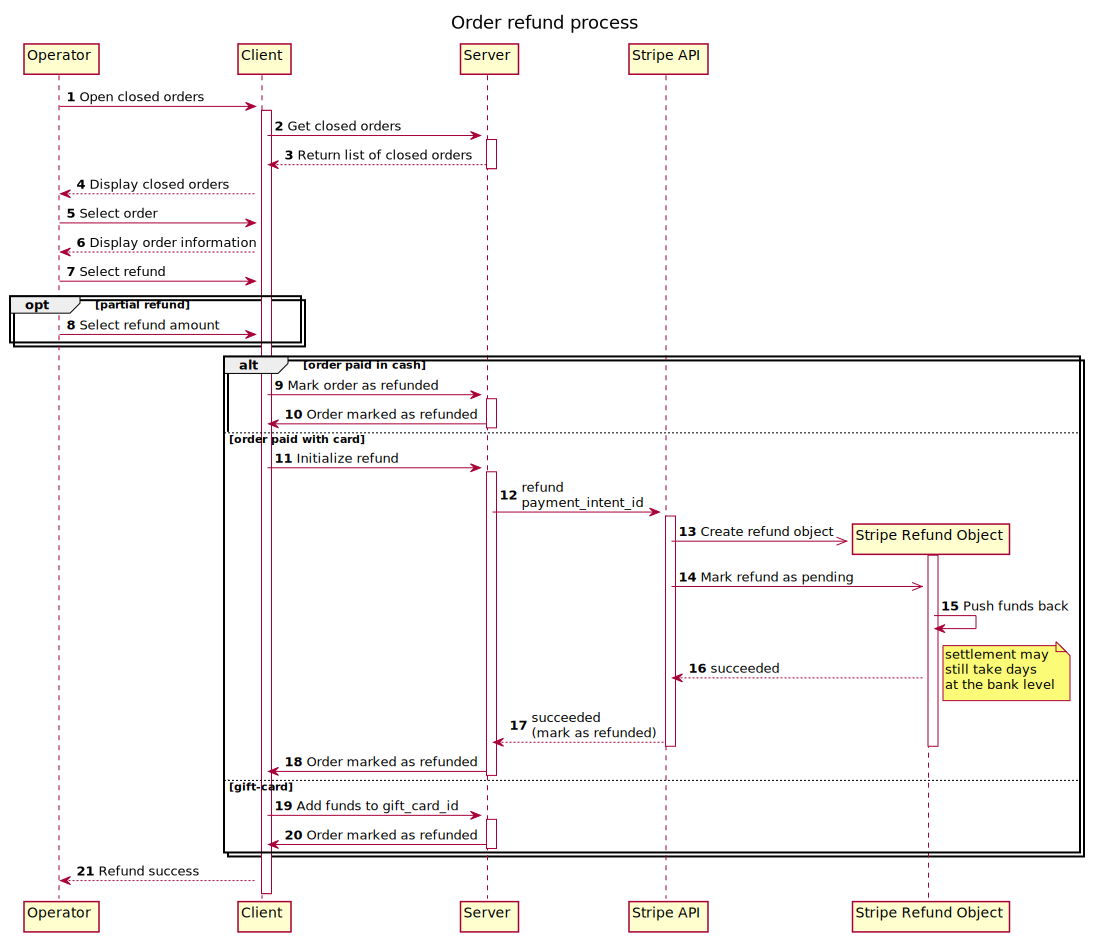
\includegraphics[width=0.9\linewidth]{PSP/lab-1/diagrams/sequence/refund.png}
        \caption{system process of refunding}
        \label{}
    \end{figure}

    \subsubsection{Inventory management}
    \paragraph{}This section describes how one manages businesses' inventory. The ability to edit the inventory amounts is available only to logged-in and authorized business owner or inventory manager.
    \paragraph{}Firstly, user has to open the inventory tab where he can see items and their number in stock that goes down automatically after an order is processed. He can also edit the numbers by pressing the Manage button and clicking on any item and typing a number in, in case of a restock, then confirming by pressing apply or cancel to reverse any changed numbers.
    \begin{figure}[H]
        \centering
        \includegraphics[width=0.9\linewidth]{PSP/lab-1/mockups/inventory.png}
        \caption{inventory tab}
        \label{}
    \end{figure}

    \subsection{Employee workflow}
    \subsubsection{Order system}
    \paragraph{}This section describes how an employee creates and modifies orders in the PoS system. This ability is available only to logged-in users.
    \paragraph{}The process starts by the employee wanting to create a new order and then new order entity with unique id is created that appears empty in the interface and employee has to add items and their amount from the item menu into it. With each add the item and its quantity is displayed on the screen in the order information. Then employee also has the option to remove any item from the displayed order, while it is not confirmed. After making sure he got everything, employee confirms the order by pressing the Proceed button and it is sent to the server, then it is considered "pending" and payment window opens up. However, before the order is confirmed there is an option to cancel it all together.
    \paragraph{}Also, there is an option to type in a giftcard code, then after pressing the Proceed button it would become active in the payment stage, or type in a special discount code to apply a discount to the whole order.
     \begin{figure}[H]
        \centering
        \includegraphics[width=0.9\linewidth]{PSP/lab-1/mockups/hometab.png}
        \caption{home tab for adding orders}
        \label{}
    \end{figure}
    
    \begin{figure}[H]
        \centering
        \includegraphics[width=0.9\linewidth]{PSP/lab-1/diagrams/sequence/order.png}
        \caption{order creation process}
        \label{}
    \end{figure}


    \subsubsection{Service appointment system}
    \paragraph{}This section describes how an employee creates and modifies order of service appointments in the PoS system. This ability is available only to logged-in users.
    \paragraph{}The process starts by the employee wanting to create a new order and then new order entity with unique id is created that appears empty in the interface and employee has to add services to it. Firstly one has to select their desired service, then time table appears based on the schedule of an employee associated with the service and they have to select date and time for their appointment, then the service is added to the order. With each add the service and its information is displayed on the screen. Then employee also has the option to remove any item from the displayed order, while it is not confirmed. After making sure he got everything, employee has to enter the customers phone number and name to be able to confirm the order. Then the order is uploaded into the server and SMS message is sent to the client about the order details. However, before the order is confirmed there is an option to cancel it all together.
    \begin{figure}[H]
        \centering
        \includegraphics[width=0.9\linewidth]{PSP/lab-1/diagrams/sequence/service-order.png}
        \caption{process of appointment registration}
        \label{}
    \end{figure}
    
    \subsubsection{Payment system}
    \paragraph{}This section describes how payments and tips are handled in the PoS system. This functionality is available only to logged-in users. Card payments are processed using Stripe services.
    \paragraph{}After taking the order and clicking the Proceed button the payment window appears, where the user is able to split the bill and select between card or cash payment for each payment or pay the full bill amount.
    \paragraph{}Also there is the possibility of adding a tip by pressing Add tip button and typing in the amount that you want to add to the bill. If a gift card code was entered previously, the amount in that card would be deducted from the bill. 
    \begin{figure}[H]
        \centering
        \includegraphics[width=0.9\linewidth]{PSP/lab-1/mockups/payments.png}
        \caption{payment window}
        \label{}
    \end{figure}

    \begin{figure}[H]
        \centering
        \includegraphics[width=0.7\linewidth]{PSP/lab-1/diagrams/sequence/payment.png}
        \caption{}
        \label{}
    \end{figure}
    
    \section{High level architecture}
    The system is split up by components (packages) that have different important responsibilities. Those smaller components add up to 5 main packages:
    \begin{itemize}
        \item Dependencies - SMS and Stripe are outside components that provide their services to our PoS system. Stripe for payments, SMS for appointment confirmation.
        \item User - the component of all employees with their schedules, roles and permissions and other people who use the system, like owner and super admin.
        \item Order - includes items and their variations(menu), inventory.
        \item Appointment - includes appointment booking and services. Connects with User package, because each service has an employee associated with it.
        \item Payments - includes taxes, discounts, giftcards.
    \end{itemize}
    
        \begin{figure}[H]
        \centering
        \includegraphics[width=0.9\linewidth]{PSP/lab-1/diagrams/architecture/highView.png}
        \caption{High level component(package) relation model}
        \label{}
        \end{figure}
        
    \section{Data model}
    \begin{figure}[H]
        \centering
        \includegraphics[width=1.0\linewidth]{PSP/lab-1/diagrams/data-model/data-model.png}
        \caption{class relations model}
        \label{data_model}
        \end{figure}
    \subsection{Data model description}
    \paragraph{}The data model describes the point of sale system. It includes description how each functionality is implemented: order process, service/appointment registration, payment system with gift-card implementation. Additionally it has a tax and discount management functionalities. 
    \paragraph{}The Figure \ref{data_model} is like a database model and relations in the diagram represent foreign keys. For example, employee relation to organization would mean that employee includes organizationId.
    \subsubsection{Permissions and enums}
    \paragraph{}Decimals are used for more precise calculations. AccessFlag in Employee is used for flexibility in permission management to each employee. Note, that specific enums can be changed based on need, for example to add a new currency or plan, etc.
    \subsubsection{Orders and payments}
    \paragraph{}Order entity could consist of multiple OrderItems that each could have a number different Variations that are connected to InventoryItems for smooth order making and inventory management. This connection checks if there is needed amount of products in stock for the order and reduces the numbers once the order is confirmed. Each Order could have a number of payments tied to it(when the check is split or multiple payment methods are chosen).
    \subsubsection{Appointments and services}
    \paragraph{}Appointment entity could consist of multiple Services offered by the business and each Service is tied to a specific Employee that is able to provide it.
    
%    \section{API Contracts for the backend endpoints}
%
%    List: ( before putting properly in .yaml)\\
%\subsection*{1. Authentication \& User Management}
%\begin{itemize}
% \item \textbf{POST} /auth/register
% \item \textbf{POST} /auth/login
% \item \textbf{POST} /auth/logout
% \item \textbf{GET} /organisations/\{organisationId\}/users
% \item \textbf{GET} /organisations/\{organisationId\}/users/\{userId\}
% \item \textbf{POST} /organisations/\{organisationId\}/users
% \item \textbf{PUT} /organisations/\{organisationId\}/users/\{userId\}
%\end{itemize}
%
%\subsection*{2. Business / Organisation Management}
%\begin{itemize}
% \item \textbf{GET} /organisations
% \item \textbf{GET} /organisations/\{organisationId\}
% \item \textbf{POST} /organisations
% \item \textbf{PUT} /organisations/\{organisationId\}
%\end{itemize}
%
%\subsection*{3. Menu / Product Management}
%\begin{itemize}
% \item \textbf{GET} /menu-items
% \item \textbf{GET} /menu-items/\{itemId\}
% \item \textbf{POST} /menu-items
% \item \textbf{PUT} /menu-items/\{itemId\}
%\end{itemize}
%
%\subsection*{4. Inventory Management}
%\begin{itemize}
% \item \textbf{GET} /inventory
% \item \textbf{GET} /inventory/\{inventoryItemId\}
% \item \textbf{POST} /inventory
% \item \textbf{PUT} /inventory/\{inventoryItemId\}
%\end{itemize}
%
%\subsection*{5. Order Management}
%\begin{itemize}
% \item \textbf{GET} /orders
% \item \textbf{GET} /orders/\{orderId\}
% \item \textbf{POST} /orders
% \item \textbf{PUT} /orders/\{orderId\}
%\end{itemize}
%
%\subsection*{6. Payment \& Refund System}
%\begin{itemize}
% \item \textbf{POST} /organisations/\{organisationId\}/orders/\{orderId\}/payments
% \item \textbf{GET} /orders/\{orderId\}/payments
% \item \textbf{POST} /orders/\{orderId\}/refund
%\end{itemize}
%
%\subsection*{7. Booking / Appointment System}
%\begin{itemize}
% \item \textbf{GET} /appointments
% \item \textbf{GET} /appointments/\{appointmentId\}
% \item \textbf{POST} /appointments
% \item \textbf{PUT} /appointments/\{appointmentId\}
%\end{itemize}
%
%\subsection*{8. Gift Cards, Discounts \& Taxes}
%\begin{itemize}
% \item \textbf{GET} /taxes
% \item \textbf{GET} /taxes/\{taxId\}
% \item \textbf{POST} /taxes
% \item \textbf{PUT} /taxes/\{taxId\}
% \item \textbf{GET} /discounts
% \item \textbf{POST} /discounts
% \item \textbf{PUT} /discounts/\{discountId\}
% \item \textbf{GET} /gift-cards/\{cardCode\}
% \item \textbf{POST} /gift-cards
% \item \textbf{PUT} /gift-cards/\{cardCode\}
%\end{itemize}
    
    
\end{document}